\section{Уравнения механики деформируемого твердого тела}
\subsection{Уравнения движения и реологические соотношения}
Для математического моделирования волновых процессов в деформируемом твердом
теле используется система динамических уравнений \cite{novatsky,sedov} в виде
\begin{eqnarray}
\label{rheology_equations}
\rho\dot{v}_i=\nabla_j\sigma_{ij}+f_i & \textrm{(уравнения движения)}\nonumber\\
\dot{\sigma}_{ij}=q_{ijkl}\dot{\varepsilon}_{kl}+F_{ij} & \textrm{(реологические
соотношения).}
\end{eqnarray}

Здесь $\rho$ – плотность среды, $v_i$ – компоненты скорости смещения,
$\sigma{ij}$ , $\varepsilon_{ij}$ -- компоненты тензоров напряжений и деформаций,
$\nabla_j$ – ковариантная производная по $j$-й координате, $f_i$ – массовые
силы, действующие на единицу объема, $F_{ij}$ -- добавочная правая часть.

В случае малых деформаций тензор скоростей деформаций $e_{ij}=\dot{\varepsilon}_{ij}$ 
выражается через компоненты скорости смещения линейным образом:
\begin{equation}
e_{ij}=\frac{1}{2}(\nabla_j v_i+\nabla_i v_j).
\end{equation}
Вид компонент тензора 4-го порядка $q_{ijkl}$ определяется реологией среды. Для 
линейно-упругого тела
\begin{eqnarray}
\label{tensor_qijkl}
q_{ijkl}=\lambda\delta_{ij}\delta{kl}+\mu(\delta_{ik}\delta_{jl}+\delta{il}
\delta{jk})\nonumber\\
F_{ij}=0.
\end{eqnarray}
В этом соотношении, которое обобщает закон Гука, $\lambda$ и $\mu$ -- параметры
Ляме, $\delta_{ij}$ -- символ Кронекера.

Для замыкания системы уравнений \ref{rheology_equations} её необходимо дополнить
уравнением состояния, определяющим зависимость плотности от напряжений:
$$\rho=\rho_0e^{\frac{p}{K}},$$
где $p=-\frac{1}{3}\sum\sigma_{kk}$ -- давление, $K=\lambda+\frac{2}{3}\mu$ --
коэффициент всестороннего сжатия.
\subsection{Матричная форма уравнений}
Уравнения \ref{rheology_equations} и \ref{tensor_qijkl} можно переписать в матричной
форме:
\begin{equation}
\label{matrix_equation}
\frac{\partial}{\partial{t}}\vec{u}^T+\mathbf{A}_x\frac{\partial}{\partial{x}}\vec{u}^T+
\mathbf{A}_y\frac{\partial}{\partial{y}}\vec{u}^T+
\mathbf{A}_z\frac{\partial}{\partial{z}}\vec{u}^T=\vec{f}^T
\end{equation}
Здесь
$\vec{u}=\{v_x,v_y,v_z,\sigma_{xx},\sigma_{yy},\sigma_{zz},\sigma_{xy},\sigma_{xz},\sigma_{yz}\}$
-- вектор искомых функций, $\vec{f}$ -- вектор правых частей той же размерности,
$x,y,z$ --  независимые пространственные переменные, $t$ -- время,
\begin{displaymath}
\mathbf{A}_x =
\left( \begin{array}{cccccccccccc}
0 & 0 & 0 & -\frac 1 \rho & 0 & 0 & 0 & 0 & 0 \\ 
0 & 0 & 0 & 0 & -\frac 1 \rho & 0 & 0 & 0 & 0 \\ 
0 & 0 & 0 & 0 & 0 & -\frac 1 \rho & 0 & 0 & 0 \\ 
-\lambda-2\mu & 0 & 0 & 0 & 0 & 0 & 0 & 0 & 0 \\ 
0 & -\mu & 0 & 0 & 0 & 0 & 0 & 0 & 0 \\ 
0 & 0 & -\mu & 0 & 0 & 0 & 0 & 0 & 0 \\ 
-\lambda & 0 & 0 & 0 & 0 & 0 & 0 & 0 & 0 \\ 
0 & 0 & 0 & 0 & 0 & 0 & 0 & 0 & 0 \\ 
-\lambda & 0 & 0 & 0 & 0 & 0 & 0 & 0 & 0  
\end{array} \right),
\end{displaymath} 
\begin{displaymath}
\mathbf{A}_y =
\left( \begin{array}{cccccccccccc}
0 & 0 & 0 & 0 & -\frac 1 \rho & 0 & 0 & 0 & 0 \\ 
0 & 0 & 0 & 0 & 0 & 0 & -\frac 1 \rho & 0 & 0 \\ 
0 & 0 & 0 & 0 & 0 & 0 & 0 & -\frac 1 \rho & 0 \\ 
0 & -\lambda & 0 & 0 & 0 & 0 & 0 & 0 & 0 \\ 
-\mu & 0 & 0 & 0 & 0 & 0 & 0 & 0 & 0 \\ 
0 & 0 & 0 & 0 & 0 & 0 & 0 & 0 & 0 \\ 
0 & -\lambda-2\mu & 0 & 0 & 0 & 0 & 0 & 0 & 0 \\ 
0 & 0 & -\mu & 0 & 0 & 0 & 0 & 0 & 0 \\ 
0 & -\lambda & 0 & 0 & 0 & 0 & 0 & 0 & 0  
\end{array} \right),
\end{displaymath}
\begin{displaymath}
\mathbf{A}_z =
\left( \begin{array}{cccccccccccc}
0 & 0 & 0 & -\frac 1 \rho & 0 & 0 & 0 & 0 & 0 \\ 
0 & 0 & 0 & 0 & -\frac 1 \rho & 0 & 0 & 0 & 0 \\ 
0 & 0 & 0 & 0 & 0 & -\frac 1 \rho & 0 & 0 & 0 \\ 
-\lambda-2\mu & 0 & 0 & 0 & 0 & 0 & 0 & 0 & 0 \\ 
0 & -\mu & 0 & 0 & 0 & 0 & 0 & 0 & 0 \\ 
0 & 0 & -\mu & 0 & 0 & 0 & 0 & 0 & 0 \\ 
-\lambda & 0 & 0 & 0 & 0 & 0 & 0 & 0 & 0 \\ 
0 & 0 & 0 & 0 & 0 & 0 & 0 & 0 & 0 \\ 
-\lambda & 0 & 0 & 0 & 0 & 0 & 0 & 0 & 0  
\end{array} \right).
\end{displaymath}
\subsection{Гиперболические свойства систем уравнений линейной упругости}
Рассмотрим одномерное уравнение вида
\begin{equation}
\frac{\partial}{\partial{t}}\vec{u}^T+\mathbf{A}\frac{\partial}{\partial{x}}\vec{u}^T=\vec{f}^T
\label{advection_equation}
\end{equation}
Если матрица $\mathbf{A}$ имеет полный набор вещественных собственных значений, 
то такое уравнение называется гиперболическим, и его решения соответствуют 
процессам, которые носят волновой характер. В этом случае справедливо разложение:
$$\mathbf{A}=\mathbf\Omega^{-1}\mathbf\Lambda\mathbf\Omega,$$
где $\mathbf\Omega$ -- матрица, составленная векторов ${\vec\omega_i}$, где
$\vec\omega_i$ есть собственные векторы матрицы $\mathbf A$,
удовлетворяющие соотношениям
$$\vec\omega_i\mathbf A=\lambda_i\vec\omega_i,$$
а $\mathbf\Lambda=diag\{\lambda_i\}$ -- диагональная матрица собственных
значений.

Домножив уравнение \ref{advection_equation} слева на $\Omega$, мы получим
уравнение
$$\frac{\partial}{\partial t}\Omega{\vec u}^T+
\Lambda\frac{\partial}{\partial x}\Omega{\vec u}^T=\Omega{\vec f}^T,$$
которое после перехода к Римановым инвариантам ${\vec v}^T=\Omega{\vec u}^T$
распадается на $n$ одномерных уравнений вида
\begin{equation}
\frac{\partial}{\partial t}{v_i}+\lambda_i\frac{\partial}{\partial
x}{v_i}={{\tilde f}_i},
\label{advection_equation_splitted}
\end{equation}
где ${{\tilde f}_i}=(\Omega{\vec f}^T)_i$.
Таким образом решение уравнения \ref{advection_equation} представляется в виде
суммы плоских волн, движущихся со скоростями $\lambda_i$.
\subsection{Метод решения исходной задачи}
Идея метода \cite{fedorenko} решения исходной задачи состоит в замене трёхмерной системы
уравнений \ref{matrix_equation} тремя одномерными системами 
\begin{equation}
\frac{\partial}{\partial t}\vec u+\mathbf{A}_x \frac{\partial}{\partial x}\vec u
= 0,
\label{matrix_equation_x}
\end{equation}
\begin{equation}
\frac{\partial}{\partial t}\vec u+\mathbf{A}_y \frac{\partial}{\partial y}\vec u
= 0,
\label{matrix_equation_y}
\end{equation}
\begin{equation}
\frac{\partial}{\partial t}\vec u+\mathbf{A}_z \frac{\partial}{\partial z}\vec u
= 0,
\label{matrix_equation_z}
\end{equation}
\begin{equation}
\frac{\partial}{\partial t}\vec u = \vec f.
\label{matrix_equation_f}
\end{equation}
Решение этих уравнений состоит из четырёх этапов: сначала во всей области
интегрирования решается уравнение \ref{matrix_equation_x}, затем полученный
результат используется для решения \ref{matrix_equation_y}, по результатам
которого решается \ref{matrix_equation_z}, и, в итоге, конечное решение
получается из уравнения \ref{matrix_equation_f}.
\subsubsection{Решение одномерной задачи}
Рассмотрим несколько подробнее метод решения однормерной задачи
\begin{equation}
\frac{\partial}{\partial t}v+\lambda \frac{\partial}{\partial x}v = 0.
\label{one_dim_eq}
\end{equation}
Для её решения предлагается использовать сеточно-характеристический метод, суть
которого состоит в следующем. Из того узла $m$ временного слоя $n+1$, в котором
требуется получить решение, опускаются характеристики.
\begin{figure}[h]
\center{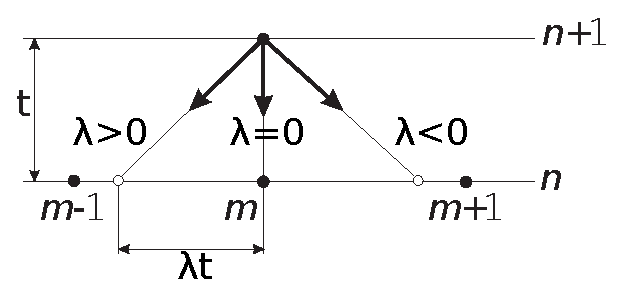
\includegraphics[width=0.3\textwidth]{eps/gcm-idea.eps}}
\caption{Принципиальная схема сеточно-характеристического метода}
\end{figure}
Из точки пересечения характеристики со слоем $n$ значение $v$ переносится в 
точку $\xi^{n+1}_m$:
$$v_i^{n+1}(\xi_m)=v^{n}_i(\xi_m-\lambda_i\tau)$$
Если характеристика не попадает точно в расчётный узел, то применяются различные
методы реконструкции значения в данной точке (в данной работе используется
интерполяция).
\subsubsection{Расчёт граничных узлов}
Метод, описанный в предыдущем пунтке, годится лишь для расчёта внутренних узлов
сетки, т.е. только в том случае, если характеристика, выпущенная из узла, не
выводит за пределы области интегрирования. В случае, когда узел является
внешним, применяется иной подход для решения задачи. Рассматриваемая система
уравнений в граничных узлах области интегрирования имеет не больше трёх
\cite{chelnokov} выводящих характеристик, поэтому для корректной постановки
задачи требуется задание граничных условий для каждого внешнего узла сетки в
количестве, равном числу выводящих характеристик. Граничные условия могут быть
нескольких видов:
\begin{itemize}
\item{свободная граница
\begin{eqnarray}
\sigma_\tau=\sigma_n=0 \nonumber
\end{eqnarray}}
\item{скольжение тел друг относительно друга 
\begin{eqnarray}
v_n=\tilde{v}_n,\nonumber\\
\sigma_n=\tilde{\sigma}_n,\nonumber\\
\sigma_\tau=\tilde{\sigma}_\tau=0 \nonumber
\end{eqnarray}}
\item{слипание тел
\begin{eqnarray}
v_n=\tilde{v}_n,\nonumber\\
v_\tau=\tilde{v}_\tau.
\end{eqnarray}}
\end{itemize}
В случае, когда узел имеет выводящие характеристики, решение опредялется
следующим образом: те компоненты искомого вектора $v^T$, которые не имеют
выводящих характеристик, считаются при помощи сеточно характеристического
метода, описанного ранее; остальные уравнения заменяются граничными
соотношениями. После этого, решается полученная СЛАУ, из которой определяются
значения всех компонент вестора $v^T$ в текущем узле.